% Created by tikzDevice version 0.12.6 on 2026-10-30 12:54:41
% !TEX encoding = UTF-8 Unicode
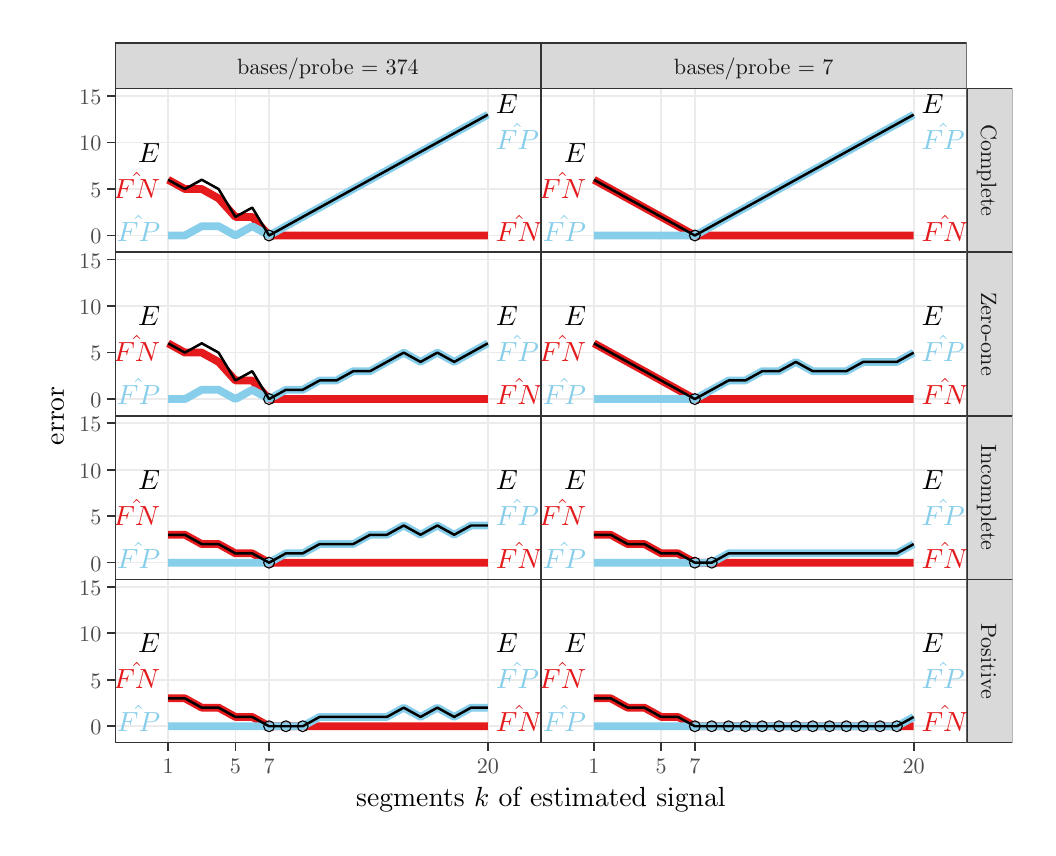
\begin{tikzpicture}[x=1pt,y=1pt]
\definecolor{fillColor}{RGB}{255,255,255}
\path[use as bounding box,fill=fillColor,fill opacity=0.00] (0,0) rectangle (361.35,289.08);
\begin{scope}
\path[clip] (  0.00,  0.00) rectangle (361.35,289.08);
\definecolor{drawColor}{RGB}{255,255,255}
\definecolor{fillColor}{RGB}{255,255,255}

\path[draw=drawColor,line width= 0.6pt,line join=round,line cap=round,fill=fillColor] (  0.00,  0.00) rectangle (361.35,289.08);
\end{scope}
\begin{scope}
\path[clip] ( 31.58,207.93) rectangle (185.45,267.04);
\definecolor{fillColor}{RGB}{255,255,255}

\path[fill=fillColor] ( 31.58,207.93) rectangle (185.45,267.04);
\definecolor{drawColor}{gray}{0.92}

\path[draw=drawColor,line width= 0.6pt,line join=round] ( 31.58,213.98) --
	(185.45,213.98);

\path[draw=drawColor,line width= 0.6pt,line join=round] ( 31.58,230.77) --
	(185.45,230.77);

\path[draw=drawColor,line width= 0.6pt,line join=round] ( 31.58,247.56) --
	(185.45,247.56);

\path[draw=drawColor,line width= 0.6pt,line join=round] ( 31.58,264.36) --
	(185.45,264.36);

\path[draw=drawColor,line width= 0.6pt,line join=round] ( 50.74,207.93) --
	( 50.74,267.04);

\path[draw=drawColor,line width= 0.6pt,line join=round] ( 75.06,207.93) --
	( 75.06,267.04);

\path[draw=drawColor,line width= 0.6pt,line join=round] ( 87.23,207.93) --
	( 87.23,267.04);

\path[draw=drawColor,line width= 0.6pt,line join=round] (166.29,207.93) --
	(166.29,267.04);
\definecolor{drawColor}{RGB}{228,26,28}

\path[draw=drawColor,line width= 2.8pt,line join=round] ( 50.74,234.13) --
	( 56.82,230.77) --
	( 62.90,230.77) --
	( 68.98,227.41) --
	( 75.06,220.70) --
	( 81.15,220.70) --
	( 87.23,213.98) --
	( 93.31,213.98) --
	( 99.39,213.98) --
	(105.47,213.98) --
	(111.55,213.98) --
	(117.64,213.98) --
	(123.72,213.98) --
	(129.80,213.98) --
	(135.88,213.98) --
	(141.96,213.98) --
	(148.04,213.98) --
	(154.13,213.98) --
	(160.21,213.98) --
	(166.29,213.98);
\definecolor{drawColor}{RGB}{135,206,235}

\path[draw=drawColor,line width= 2.8pt,line join=round] ( 50.74,213.98) --
	( 56.82,213.98) --
	( 62.90,217.34) --
	( 68.98,217.34) --
	( 75.06,213.98) --
	( 81.15,217.34) --
	( 87.23,213.98) --
	( 93.31,217.34) --
	( 99.39,220.70) --
	(105.47,224.06) --
	(111.55,227.41) --
	(117.64,230.77) --
	(123.72,234.13) --
	(129.80,237.49) --
	(135.88,240.85) --
	(141.96,244.21) --
	(148.04,247.56) --
	(154.13,250.92) --
	(160.21,254.28) --
	(166.29,257.64);
\definecolor{drawColor}{RGB}{0,0,0}

\path[draw=drawColor,line width= 0.9pt,line join=round] ( 50.74,234.13) --
	( 56.82,230.77) --
	( 62.90,234.13) --
	( 68.98,230.77) --
	( 75.06,220.70) --
	( 81.15,224.06) --
	( 87.23,213.98) --
	( 93.31,217.34) --
	( 99.39,220.70) --
	(105.47,224.06) --
	(111.55,227.41) --
	(117.64,230.77) --
	(123.72,234.13) --
	(129.80,237.49) --
	(135.88,240.85) --
	(141.96,244.21) --
	(148.04,247.56) --
	(154.13,250.92) --
	(160.21,254.28) --
	(166.29,257.64);

\path[draw=drawColor,line width= 0.4pt,line join=round,line cap=round] ( 87.23,213.98) circle (  1.96);
\end{scope}
\begin{scope}
\path[clip] ( 31.58,207.93) rectangle (185.45,267.04);
\definecolor{drawColor}{RGB}{228,26,28}

\node[text=drawColor,anchor=base east,inner sep=0pt, outer sep=0pt, scale=  1.00] at ( 47.89,227.50) {$\hat{\text{FN}}$};

\node[text=drawColor,anchor=base west,inner sep=0pt, outer sep=0pt, scale=  1.00] at (169.14,211.94) {$\hat{\text{FN}}$};
\definecolor{drawColor}{RGB}{0,0,0}

\node[text=drawColor,anchor=base east,inner sep=0pt, outer sep=0pt, scale=  1.00] at ( 47.89,240.48) {$E$};

\node[text=drawColor,anchor=base west,inner sep=0pt, outer sep=0pt, scale=  1.00] at (169.14,258.07) {$E$};
\definecolor{drawColor}{RGB}{135,206,235}

\node[text=drawColor,anchor=base east,inner sep=0pt, outer sep=0pt, scale=  1.00] at ( 47.89,211.94) {$\hat{\text{FP}}$};

\node[text=drawColor,anchor=base west,inner sep=0pt, outer sep=0pt, scale=  1.00] at (169.14,245.08) {$\hat{\text{FP}}$};
\definecolor{drawColor}{gray}{0.20}

\path[draw=drawColor,line width= 0.6pt,line join=round,line cap=round] ( 31.58,207.93) rectangle (185.45,267.04);
\end{scope}
\begin{scope}
\path[clip] ( 31.58,148.83) rectangle (185.45,207.93);
\definecolor{fillColor}{RGB}{255,255,255}

\path[fill=fillColor] ( 31.58,148.83) rectangle (185.45,207.93);
\definecolor{drawColor}{gray}{0.92}

\path[draw=drawColor,line width= 0.6pt,line join=round] ( 31.58,154.87) --
	(185.45,154.87);

\path[draw=drawColor,line width= 0.6pt,line join=round] ( 31.58,171.66) --
	(185.45,171.66);

\path[draw=drawColor,line width= 0.6pt,line join=round] ( 31.58,188.46) --
	(185.45,188.46);

\path[draw=drawColor,line width= 0.6pt,line join=round] ( 31.58,205.25) --
	(185.45,205.25);

\path[draw=drawColor,line width= 0.6pt,line join=round] ( 50.74,148.83) --
	( 50.74,207.93);

\path[draw=drawColor,line width= 0.6pt,line join=round] ( 75.06,148.83) --
	( 75.06,207.93);

\path[draw=drawColor,line width= 0.6pt,line join=round] ( 87.23,148.83) --
	( 87.23,207.93);

\path[draw=drawColor,line width= 0.6pt,line join=round] (166.29,148.83) --
	(166.29,207.93);
\definecolor{drawColor}{RGB}{228,26,28}

\path[draw=drawColor,line width= 2.8pt,line join=round] ( 50.74,175.02) --
	( 56.82,171.66) --
	( 62.90,171.66) --
	( 68.98,168.30) --
	( 75.06,161.59) --
	( 81.15,161.59) --
	( 87.23,154.87) --
	( 93.31,154.87) --
	( 99.39,154.87) --
	(105.47,154.87) --
	(111.55,154.87) --
	(117.64,154.87) --
	(123.72,154.87) --
	(129.80,154.87) --
	(135.88,154.87) --
	(141.96,154.87) --
	(148.04,154.87) --
	(154.13,154.87) --
	(160.21,154.87) --
	(166.29,154.87);
\definecolor{drawColor}{RGB}{135,206,235}

\path[draw=drawColor,line width= 2.8pt,line join=round] ( 50.74,154.87) --
	( 56.82,154.87) --
	( 62.90,158.23) --
	( 68.98,158.23) --
	( 75.06,154.87) --
	( 81.15,158.23) --
	( 87.23,154.87) --
	( 93.31,158.23) --
	( 99.39,158.23) --
	(105.47,161.59) --
	(111.55,161.59) --
	(117.64,164.95) --
	(123.72,164.95) --
	(129.80,168.30) --
	(135.88,171.66) --
	(141.96,168.30) --
	(148.04,171.66) --
	(154.13,168.30) --
	(160.21,171.66) --
	(166.29,175.02);
\definecolor{drawColor}{RGB}{0,0,0}

\path[draw=drawColor,line width= 0.9pt,line join=round] ( 50.74,175.02) --
	( 56.82,171.66) --
	( 62.90,175.02) --
	( 68.98,171.66) --
	( 75.06,161.59) --
	( 81.15,164.95) --
	( 87.23,154.87) --
	( 93.31,158.23) --
	( 99.39,158.23) --
	(105.47,161.59) --
	(111.55,161.59) --
	(117.64,164.95) --
	(123.72,164.95) --
	(129.80,168.30) --
	(135.88,171.66) --
	(141.96,168.30) --
	(148.04,171.66) --
	(154.13,168.30) --
	(160.21,171.66) --
	(166.29,175.02);

\path[draw=drawColor,line width= 0.4pt,line join=round,line cap=round] ( 87.23,154.87) circle (  1.96);
\end{scope}
\begin{scope}
\path[clip] ( 31.58,148.83) rectangle (185.45,207.93);
\definecolor{drawColor}{RGB}{228,26,28}

\node[text=drawColor,anchor=base east,inner sep=0pt, outer sep=0pt, scale=  1.00] at ( 47.89,168.39) {$\hat{\text{FN}}$};

\node[text=drawColor,anchor=base west,inner sep=0pt, outer sep=0pt, scale=  1.00] at (169.14,152.83) {$\hat{\text{FN}}$};
\definecolor{drawColor}{RGB}{0,0,0}

\node[text=drawColor,anchor=base east,inner sep=0pt, outer sep=0pt, scale=  1.00] at ( 47.89,181.38) {$E$};

\node[text=drawColor,anchor=base west,inner sep=0pt, outer sep=0pt, scale=  1.00] at (169.14,181.38) {$E$};
\definecolor{drawColor}{RGB}{135,206,235}

\node[text=drawColor,anchor=base east,inner sep=0pt, outer sep=0pt, scale=  1.00] at ( 47.89,152.83) {$\hat{\text{FP}}$};

\node[text=drawColor,anchor=base west,inner sep=0pt, outer sep=0pt, scale=  1.00] at (169.14,168.39) {$\hat{\text{FP}}$};
\definecolor{drawColor}{gray}{0.20}

\path[draw=drawColor,line width= 0.6pt,line join=round,line cap=round] ( 31.58,148.83) rectangle (185.45,207.93);
\end{scope}
\begin{scope}
\path[clip] ( 31.58, 89.72) rectangle (185.45,148.83);
\definecolor{fillColor}{RGB}{255,255,255}

\path[fill=fillColor] ( 31.58, 89.72) rectangle (185.45,148.83);
\definecolor{drawColor}{gray}{0.92}

\path[draw=drawColor,line width= 0.6pt,line join=round] ( 31.58, 95.76) --
	(185.45, 95.76);

\path[draw=drawColor,line width= 0.6pt,line join=round] ( 31.58,112.55) --
	(185.45,112.55);

\path[draw=drawColor,line width= 0.6pt,line join=round] ( 31.58,129.35) --
	(185.45,129.35);

\path[draw=drawColor,line width= 0.6pt,line join=round] ( 31.58,146.14) --
	(185.45,146.14);

\path[draw=drawColor,line width= 0.6pt,line join=round] ( 50.74, 89.72) --
	( 50.74,148.83);

\path[draw=drawColor,line width= 0.6pt,line join=round] ( 75.06, 89.72) --
	( 75.06,148.83);

\path[draw=drawColor,line width= 0.6pt,line join=round] ( 87.23, 89.72) --
	( 87.23,148.83);

\path[draw=drawColor,line width= 0.6pt,line join=round] (166.29, 89.72) --
	(166.29,148.83);
\definecolor{drawColor}{RGB}{228,26,28}

\path[draw=drawColor,line width= 2.8pt,line join=round] ( 50.74,105.84) --
	( 56.82,105.84) --
	( 62.90,102.48) --
	( 68.98,102.48) --
	( 75.06, 99.12) --
	( 81.15, 99.12) --
	( 87.23, 95.76) --
	( 93.31, 95.76) --
	( 99.39, 95.76) --
	(105.47, 95.76) --
	(111.55, 95.76) --
	(117.64, 95.76) --
	(123.72, 95.76) --
	(129.80, 95.76) --
	(135.88, 95.76) --
	(141.96, 95.76) --
	(148.04, 95.76) --
	(154.13, 95.76) --
	(160.21, 95.76) --
	(166.29, 95.76);
\definecolor{drawColor}{RGB}{135,206,235}

\path[draw=drawColor,line width= 2.8pt,line join=round] ( 50.74, 95.76) --
	( 56.82, 95.76) --
	( 62.90, 95.76) --
	( 68.98, 95.76) --
	( 75.06, 95.76) --
	( 81.15, 95.76) --
	( 87.23, 95.76) --
	( 93.31, 99.12) --
	( 99.39, 99.12) --
	(105.47,102.48) --
	(111.55,102.48) --
	(117.64,102.48) --
	(123.72,105.84) --
	(129.80,105.84) --
	(135.88,109.19) --
	(141.96,105.84) --
	(148.04,109.19) --
	(154.13,105.84) --
	(160.21,109.19) --
	(166.29,109.19);
\definecolor{drawColor}{RGB}{0,0,0}

\path[draw=drawColor,line width= 0.9pt,line join=round] ( 50.74,105.84) --
	( 56.82,105.84) --
	( 62.90,102.48) --
	( 68.98,102.48) --
	( 75.06, 99.12) --
	( 81.15, 99.12) --
	( 87.23, 95.76) --
	( 93.31, 99.12) --
	( 99.39, 99.12) --
	(105.47,102.48) --
	(111.55,102.48) --
	(117.64,102.48) --
	(123.72,105.84) --
	(129.80,105.84) --
	(135.88,109.19) --
	(141.96,105.84) --
	(148.04,109.19) --
	(154.13,105.84) --
	(160.21,109.19) --
	(166.29,109.19);

\path[draw=drawColor,line width= 0.4pt,line join=round,line cap=round] ( 87.23, 95.76) circle (  1.96);
\end{scope}
\begin{scope}
\path[clip] ( 31.58, 89.72) rectangle (185.45,148.83);
\definecolor{drawColor}{RGB}{228,26,28}

\node[text=drawColor,anchor=base east,inner sep=0pt, outer sep=0pt, scale=  1.00] at ( 47.89,109.28) {$\hat{\text{FN}}$};

\node[text=drawColor,anchor=base west,inner sep=0pt, outer sep=0pt, scale=  1.00] at (169.14, 93.72) {$\hat{\text{FN}}$};
\definecolor{drawColor}{RGB}{0,0,0}

\node[text=drawColor,anchor=base east,inner sep=0pt, outer sep=0pt, scale=  1.00] at ( 47.89,122.27) {$E$};

\node[text=drawColor,anchor=base west,inner sep=0pt, outer sep=0pt, scale=  1.00] at (169.14,122.27) {$E$};
\definecolor{drawColor}{RGB}{135,206,235}

\node[text=drawColor,anchor=base east,inner sep=0pt, outer sep=0pt, scale=  1.00] at ( 47.89, 93.72) {$\hat{\text{FP}}$};

\node[text=drawColor,anchor=base west,inner sep=0pt, outer sep=0pt, scale=  1.00] at (169.14,109.28) {$\hat{\text{FP}}$};
\definecolor{drawColor}{gray}{0.20}

\path[draw=drawColor,line width= 0.6pt,line join=round,line cap=round] ( 31.58, 89.72) rectangle (185.45,148.83);
\end{scope}
\begin{scope}
\path[clip] ( 31.58, 30.61) rectangle (185.45, 89.72);
\definecolor{fillColor}{RGB}{255,255,255}

\path[fill=fillColor] ( 31.58, 30.61) rectangle (185.45, 89.72);
\definecolor{drawColor}{gray}{0.92}

\path[draw=drawColor,line width= 0.6pt,line join=round] ( 31.58, 36.65) --
	(185.45, 36.65);

\path[draw=drawColor,line width= 0.6pt,line join=round] ( 31.58, 53.44) --
	(185.45, 53.44);

\path[draw=drawColor,line width= 0.6pt,line join=round] ( 31.58, 70.24) --
	(185.45, 70.24);

\path[draw=drawColor,line width= 0.6pt,line join=round] ( 31.58, 87.03) --
	(185.45, 87.03);

\path[draw=drawColor,line width= 0.6pt,line join=round] ( 50.74, 30.61) --
	( 50.74, 89.72);

\path[draw=drawColor,line width= 0.6pt,line join=round] ( 75.06, 30.61) --
	( 75.06, 89.72);

\path[draw=drawColor,line width= 0.6pt,line join=round] ( 87.23, 30.61) --
	( 87.23, 89.72);

\path[draw=drawColor,line width= 0.6pt,line join=round] (166.29, 30.61) --
	(166.29, 89.72);
\definecolor{drawColor}{RGB}{228,26,28}

\path[draw=drawColor,line width= 2.8pt,line join=round] ( 50.74, 46.73) --
	( 56.82, 46.73) --
	( 62.90, 43.37) --
	( 68.98, 43.37) --
	( 75.06, 40.01) --
	( 81.15, 40.01) --
	( 87.23, 36.65) --
	( 93.31, 36.65) --
	( 99.39, 36.65) --
	(105.47, 36.65) --
	(111.55, 36.65) --
	(117.64, 36.65) --
	(123.72, 36.65) --
	(129.80, 36.65) --
	(135.88, 36.65) --
	(141.96, 36.65) --
	(148.04, 36.65) --
	(154.13, 36.65) --
	(160.21, 36.65) --
	(166.29, 36.65);
\definecolor{drawColor}{RGB}{135,206,235}

\path[draw=drawColor,line width= 2.8pt,line join=round] ( 50.74, 36.65) --
	( 56.82, 36.65) --
	( 62.90, 36.65) --
	( 68.98, 36.65) --
	( 75.06, 36.65) --
	( 81.15, 36.65) --
	( 87.23, 36.65) --
	( 93.31, 36.65) --
	( 99.39, 36.65) --
	(105.47, 40.01) --
	(111.55, 40.01) --
	(117.64, 40.01) --
	(123.72, 40.01) --
	(129.80, 40.01) --
	(135.88, 43.37) --
	(141.96, 40.01) --
	(148.04, 43.37) --
	(154.13, 40.01) --
	(160.21, 43.37) --
	(166.29, 43.37);
\definecolor{drawColor}{RGB}{0,0,0}

\path[draw=drawColor,line width= 0.9pt,line join=round] ( 50.74, 46.73) --
	( 56.82, 46.73) --
	( 62.90, 43.37) --
	( 68.98, 43.37) --
	( 75.06, 40.01) --
	( 81.15, 40.01) --
	( 87.23, 36.65) --
	( 93.31, 36.65) --
	( 99.39, 36.65) --
	(105.47, 40.01) --
	(111.55, 40.01) --
	(117.64, 40.01) --
	(123.72, 40.01) --
	(129.80, 40.01) --
	(135.88, 43.37) --
	(141.96, 40.01) --
	(148.04, 43.37) --
	(154.13, 40.01) --
	(160.21, 43.37) --
	(166.29, 43.37);

\path[draw=drawColor,line width= 0.4pt,line join=round,line cap=round] ( 87.23, 36.65) circle (  1.96);

\path[draw=drawColor,line width= 0.4pt,line join=round,line cap=round] ( 93.31, 36.65) circle (  1.96);

\path[draw=drawColor,line width= 0.4pt,line join=round,line cap=round] ( 99.39, 36.65) circle (  1.96);
\end{scope}
\begin{scope}
\path[clip] ( 31.58, 30.61) rectangle (185.45, 89.72);
\definecolor{drawColor}{RGB}{228,26,28}

\node[text=drawColor,anchor=base east,inner sep=0pt, outer sep=0pt, scale=  1.00] at ( 47.89, 50.17) {$\hat{\text{FN}}$};

\node[text=drawColor,anchor=base west,inner sep=0pt, outer sep=0pt, scale=  1.00] at (169.14, 34.61) {$\hat{\text{FN}}$};
\definecolor{drawColor}{RGB}{0,0,0}

\node[text=drawColor,anchor=base east,inner sep=0pt, outer sep=0pt, scale=  1.00] at ( 47.89, 63.16) {$E$};

\node[text=drawColor,anchor=base west,inner sep=0pt, outer sep=0pt, scale=  1.00] at (169.14, 63.16) {$E$};
\definecolor{drawColor}{RGB}{135,206,235}

\node[text=drawColor,anchor=base east,inner sep=0pt, outer sep=0pt, scale=  1.00] at ( 47.89, 34.61) {$\hat{\text{FP}}$};

\node[text=drawColor,anchor=base west,inner sep=0pt, outer sep=0pt, scale=  1.00] at (169.14, 50.17) {$\hat{\text{FP}}$};
\definecolor{drawColor}{gray}{0.20}

\path[draw=drawColor,line width= 0.6pt,line join=round,line cap=round] ( 31.58, 30.61) rectangle (185.45, 89.72);
\end{scope}
\begin{scope}
\path[clip] (185.45,207.93) rectangle (339.31,267.04);
\definecolor{fillColor}{RGB}{255,255,255}

\path[fill=fillColor] (185.45,207.93) rectangle (339.31,267.04);
\definecolor{drawColor}{gray}{0.92}

\path[draw=drawColor,line width= 0.6pt,line join=round] (185.45,213.98) --
	(339.31,213.98);

\path[draw=drawColor,line width= 0.6pt,line join=round] (185.45,230.77) --
	(339.31,230.77);

\path[draw=drawColor,line width= 0.6pt,line join=round] (185.45,247.56) --
	(339.31,247.56);

\path[draw=drawColor,line width= 0.6pt,line join=round] (185.45,264.36) --
	(339.31,264.36);

\path[draw=drawColor,line width= 0.6pt,line join=round] (204.60,207.93) --
	(204.60,267.04);

\path[draw=drawColor,line width= 0.6pt,line join=round] (228.93,207.93) --
	(228.93,267.04);

\path[draw=drawColor,line width= 0.6pt,line join=round] (241.09,207.93) --
	(241.09,267.04);

\path[draw=drawColor,line width= 0.6pt,line join=round] (320.16,207.93) --
	(320.16,267.04);
\definecolor{drawColor}{RGB}{228,26,28}

\path[draw=drawColor,line width= 2.8pt,line join=round] (204.60,234.13) --
	(210.69,230.77) --
	(216.77,227.41) --
	(222.85,224.06) --
	(228.93,220.70) --
	(235.01,217.34) --
	(241.09,213.98) --
	(247.18,213.98) --
	(253.26,213.98) --
	(259.34,213.98) --
	(265.42,213.98) --
	(271.50,213.98) --
	(277.58,213.98) --
	(283.67,213.98) --
	(289.75,213.98) --
	(295.83,213.98) --
	(301.91,213.98) --
	(307.99,213.98) --
	(314.07,213.98) --
	(320.16,213.98);
\definecolor{drawColor}{RGB}{135,206,235}

\path[draw=drawColor,line width= 2.8pt,line join=round] (204.60,213.98) --
	(210.69,213.98) --
	(216.77,213.98) --
	(222.85,213.98) --
	(228.93,213.98) --
	(235.01,213.98) --
	(241.09,213.98) --
	(247.18,217.34) --
	(253.26,220.70) --
	(259.34,224.06) --
	(265.42,227.41) --
	(271.50,230.77) --
	(277.58,234.13) --
	(283.67,237.49) --
	(289.75,240.85) --
	(295.83,244.21) --
	(301.91,247.56) --
	(307.99,250.92) --
	(314.07,254.28) --
	(320.16,257.64);
\definecolor{drawColor}{RGB}{0,0,0}

\path[draw=drawColor,line width= 0.9pt,line join=round] (204.60,234.13) --
	(210.69,230.77) --
	(216.77,227.41) --
	(222.85,224.06) --
	(228.93,220.70) --
	(235.01,217.34) --
	(241.09,213.98) --
	(247.18,217.34) --
	(253.26,220.70) --
	(259.34,224.06) --
	(265.42,227.41) --
	(271.50,230.77) --
	(277.58,234.13) --
	(283.67,237.49) --
	(289.75,240.85) --
	(295.83,244.21) --
	(301.91,247.56) --
	(307.99,250.92) --
	(314.07,254.28) --
	(320.16,257.64);

\path[draw=drawColor,line width= 0.4pt,line join=round,line cap=round] (241.09,213.98) circle (  1.96);
\end{scope}
\begin{scope}
\path[clip] (185.45,207.93) rectangle (339.31,267.04);
\definecolor{drawColor}{RGB}{228,26,28}

\node[text=drawColor,anchor=base east,inner sep=0pt, outer sep=0pt, scale=  1.00] at (201.76,227.50) {$\hat{\text{FN}}$};

\node[text=drawColor,anchor=base west,inner sep=0pt, outer sep=0pt, scale=  1.00] at (323.00,211.94) {$\hat{\text{FN}}$};
\definecolor{drawColor}{RGB}{0,0,0}

\node[text=drawColor,anchor=base east,inner sep=0pt, outer sep=0pt, scale=  1.00] at (201.76,240.48) {$E$};

\node[text=drawColor,anchor=base west,inner sep=0pt, outer sep=0pt, scale=  1.00] at (323.00,258.07) {$E$};
\definecolor{drawColor}{RGB}{135,206,235}

\node[text=drawColor,anchor=base east,inner sep=0pt, outer sep=0pt, scale=  1.00] at (201.76,211.94) {$\hat{\text{FP}}$};

\node[text=drawColor,anchor=base west,inner sep=0pt, outer sep=0pt, scale=  1.00] at (323.00,245.08) {$\hat{\text{FP}}$};
\definecolor{drawColor}{gray}{0.20}

\path[draw=drawColor,line width= 0.6pt,line join=round,line cap=round] (185.45,207.93) rectangle (339.31,267.04);
\end{scope}
\begin{scope}
\path[clip] (185.45,148.83) rectangle (339.31,207.93);
\definecolor{fillColor}{RGB}{255,255,255}

\path[fill=fillColor] (185.45,148.83) rectangle (339.31,207.93);
\definecolor{drawColor}{gray}{0.92}

\path[draw=drawColor,line width= 0.6pt,line join=round] (185.45,154.87) --
	(339.31,154.87);

\path[draw=drawColor,line width= 0.6pt,line join=round] (185.45,171.66) --
	(339.31,171.66);

\path[draw=drawColor,line width= 0.6pt,line join=round] (185.45,188.46) --
	(339.31,188.46);

\path[draw=drawColor,line width= 0.6pt,line join=round] (185.45,205.25) --
	(339.31,205.25);

\path[draw=drawColor,line width= 0.6pt,line join=round] (204.60,148.83) --
	(204.60,207.93);

\path[draw=drawColor,line width= 0.6pt,line join=round] (228.93,148.83) --
	(228.93,207.93);

\path[draw=drawColor,line width= 0.6pt,line join=round] (241.09,148.83) --
	(241.09,207.93);

\path[draw=drawColor,line width= 0.6pt,line join=round] (320.16,148.83) --
	(320.16,207.93);
\definecolor{drawColor}{RGB}{228,26,28}

\path[draw=drawColor,line width= 2.8pt,line join=round] (204.60,175.02) --
	(210.69,171.66) --
	(216.77,168.30) --
	(222.85,164.95) --
	(228.93,161.59) --
	(235.01,158.23) --
	(241.09,154.87) --
	(247.18,154.87) --
	(253.26,154.87) --
	(259.34,154.87) --
	(265.42,154.87) --
	(271.50,154.87) --
	(277.58,154.87) --
	(283.67,154.87) --
	(289.75,154.87) --
	(295.83,154.87) --
	(301.91,154.87) --
	(307.99,154.87) --
	(314.07,154.87) --
	(320.16,154.87);
\definecolor{drawColor}{RGB}{135,206,235}

\path[draw=drawColor,line width= 2.8pt,line join=round] (204.60,154.87) --
	(210.69,154.87) --
	(216.77,154.87) --
	(222.85,154.87) --
	(228.93,154.87) --
	(235.01,154.87) --
	(241.09,154.87) --
	(247.18,158.23) --
	(253.26,161.59) --
	(259.34,161.59) --
	(265.42,164.95) --
	(271.50,164.95) --
	(277.58,168.30) --
	(283.67,164.95) --
	(289.75,164.95) --
	(295.83,164.95) --
	(301.91,168.30) --
	(307.99,168.30) --
	(314.07,168.30) --
	(320.16,171.66);
\definecolor{drawColor}{RGB}{0,0,0}

\path[draw=drawColor,line width= 0.9pt,line join=round] (204.60,175.02) --
	(210.69,171.66) --
	(216.77,168.30) --
	(222.85,164.95) --
	(228.93,161.59) --
	(235.01,158.23) --
	(241.09,154.87) --
	(247.18,158.23) --
	(253.26,161.59) --
	(259.34,161.59) --
	(265.42,164.95) --
	(271.50,164.95) --
	(277.58,168.30) --
	(283.67,164.95) --
	(289.75,164.95) --
	(295.83,164.95) --
	(301.91,168.30) --
	(307.99,168.30) --
	(314.07,168.30) --
	(320.16,171.66);

\path[draw=drawColor,line width= 0.4pt,line join=round,line cap=round] (241.09,154.87) circle (  1.96);
\end{scope}
\begin{scope}
\path[clip] (185.45,148.83) rectangle (339.31,207.93);
\definecolor{drawColor}{RGB}{228,26,28}

\node[text=drawColor,anchor=base east,inner sep=0pt, outer sep=0pt, scale=  1.00] at (201.76,168.39) {$\hat{\text{FN}}$};

\node[text=drawColor,anchor=base west,inner sep=0pt, outer sep=0pt, scale=  1.00] at (323.00,152.83) {$\hat{\text{FN}}$};
\definecolor{drawColor}{RGB}{0,0,0}

\node[text=drawColor,anchor=base east,inner sep=0pt, outer sep=0pt, scale=  1.00] at (201.76,181.38) {$E$};

\node[text=drawColor,anchor=base west,inner sep=0pt, outer sep=0pt, scale=  1.00] at (323.00,181.38) {$E$};
\definecolor{drawColor}{RGB}{135,206,235}

\node[text=drawColor,anchor=base east,inner sep=0pt, outer sep=0pt, scale=  1.00] at (201.76,152.83) {$\hat{\text{FP}}$};

\node[text=drawColor,anchor=base west,inner sep=0pt, outer sep=0pt, scale=  1.00] at (323.00,168.39) {$\hat{\text{FP}}$};
\definecolor{drawColor}{gray}{0.20}

\path[draw=drawColor,line width= 0.6pt,line join=round,line cap=round] (185.45,148.83) rectangle (339.31,207.93);
\end{scope}
\begin{scope}
\path[clip] (185.45, 89.72) rectangle (339.31,148.83);
\definecolor{fillColor}{RGB}{255,255,255}

\path[fill=fillColor] (185.45, 89.72) rectangle (339.31,148.83);
\definecolor{drawColor}{gray}{0.92}

\path[draw=drawColor,line width= 0.6pt,line join=round] (185.45, 95.76) --
	(339.31, 95.76);

\path[draw=drawColor,line width= 0.6pt,line join=round] (185.45,112.55) --
	(339.31,112.55);

\path[draw=drawColor,line width= 0.6pt,line join=round] (185.45,129.35) --
	(339.31,129.35);

\path[draw=drawColor,line width= 0.6pt,line join=round] (185.45,146.14) --
	(339.31,146.14);

\path[draw=drawColor,line width= 0.6pt,line join=round] (204.60, 89.72) --
	(204.60,148.83);

\path[draw=drawColor,line width= 0.6pt,line join=round] (228.93, 89.72) --
	(228.93,148.83);

\path[draw=drawColor,line width= 0.6pt,line join=round] (241.09, 89.72) --
	(241.09,148.83);

\path[draw=drawColor,line width= 0.6pt,line join=round] (320.16, 89.72) --
	(320.16,148.83);
\definecolor{drawColor}{RGB}{228,26,28}

\path[draw=drawColor,line width= 2.8pt,line join=round] (204.60,105.84) --
	(210.69,105.84) --
	(216.77,102.48) --
	(222.85,102.48) --
	(228.93, 99.12) --
	(235.01, 99.12) --
	(241.09, 95.76) --
	(247.18, 95.76) --
	(253.26, 95.76) --
	(259.34, 95.76) --
	(265.42, 95.76) --
	(271.50, 95.76) --
	(277.58, 95.76) --
	(283.67, 95.76) --
	(289.75, 95.76) --
	(295.83, 95.76) --
	(301.91, 95.76) --
	(307.99, 95.76) --
	(314.07, 95.76) --
	(320.16, 95.76);
\definecolor{drawColor}{RGB}{135,206,235}

\path[draw=drawColor,line width= 2.8pt,line join=round] (204.60, 95.76) --
	(210.69, 95.76) --
	(216.77, 95.76) --
	(222.85, 95.76) --
	(228.93, 95.76) --
	(235.01, 95.76) --
	(241.09, 95.76) --
	(247.18, 95.76) --
	(253.26, 99.12) --
	(259.34, 99.12) --
	(265.42, 99.12) --
	(271.50, 99.12) --
	(277.58, 99.12) --
	(283.67, 99.12) --
	(289.75, 99.12) --
	(295.83, 99.12) --
	(301.91, 99.12) --
	(307.99, 99.12) --
	(314.07, 99.12) --
	(320.16,102.48);
\definecolor{drawColor}{RGB}{0,0,0}

\path[draw=drawColor,line width= 0.9pt,line join=round] (204.60,105.84) --
	(210.69,105.84) --
	(216.77,102.48) --
	(222.85,102.48) --
	(228.93, 99.12) --
	(235.01, 99.12) --
	(241.09, 95.76) --
	(247.18, 95.76) --
	(253.26, 99.12) --
	(259.34, 99.12) --
	(265.42, 99.12) --
	(271.50, 99.12) --
	(277.58, 99.12) --
	(283.67, 99.12) --
	(289.75, 99.12) --
	(295.83, 99.12) --
	(301.91, 99.12) --
	(307.99, 99.12) --
	(314.07, 99.12) --
	(320.16,102.48);

\path[draw=drawColor,line width= 0.4pt,line join=round,line cap=round] (241.09, 95.76) circle (  1.96);

\path[draw=drawColor,line width= 0.4pt,line join=round,line cap=round] (247.18, 95.76) circle (  1.96);
\end{scope}
\begin{scope}
\path[clip] (185.45, 89.72) rectangle (339.31,148.83);
\definecolor{drawColor}{RGB}{228,26,28}

\node[text=drawColor,anchor=base east,inner sep=0pt, outer sep=0pt, scale=  1.00] at (201.76,109.28) {$\hat{\text{FN}}$};

\node[text=drawColor,anchor=base west,inner sep=0pt, outer sep=0pt, scale=  1.00] at (323.00, 93.72) {$\hat{\text{FN}}$};
\definecolor{drawColor}{RGB}{0,0,0}

\node[text=drawColor,anchor=base east,inner sep=0pt, outer sep=0pt, scale=  1.00] at (201.76,122.27) {$E$};

\node[text=drawColor,anchor=base west,inner sep=0pt, outer sep=0pt, scale=  1.00] at (323.00,122.27) {$E$};
\definecolor{drawColor}{RGB}{135,206,235}

\node[text=drawColor,anchor=base east,inner sep=0pt, outer sep=0pt, scale=  1.00] at (201.76, 93.72) {$\hat{\text{FP}}$};

\node[text=drawColor,anchor=base west,inner sep=0pt, outer sep=0pt, scale=  1.00] at (323.00,109.28) {$\hat{\text{FP}}$};
\definecolor{drawColor}{gray}{0.20}

\path[draw=drawColor,line width= 0.6pt,line join=round,line cap=round] (185.45, 89.72) rectangle (339.31,148.83);
\end{scope}
\begin{scope}
\path[clip] (185.45, 30.61) rectangle (339.31, 89.72);
\definecolor{fillColor}{RGB}{255,255,255}

\path[fill=fillColor] (185.45, 30.61) rectangle (339.31, 89.72);
\definecolor{drawColor}{gray}{0.92}

\path[draw=drawColor,line width= 0.6pt,line join=round] (185.45, 36.65) --
	(339.31, 36.65);

\path[draw=drawColor,line width= 0.6pt,line join=round] (185.45, 53.44) --
	(339.31, 53.44);

\path[draw=drawColor,line width= 0.6pt,line join=round] (185.45, 70.24) --
	(339.31, 70.24);

\path[draw=drawColor,line width= 0.6pt,line join=round] (185.45, 87.03) --
	(339.31, 87.03);

\path[draw=drawColor,line width= 0.6pt,line join=round] (204.60, 30.61) --
	(204.60, 89.72);

\path[draw=drawColor,line width= 0.6pt,line join=round] (228.93, 30.61) --
	(228.93, 89.72);

\path[draw=drawColor,line width= 0.6pt,line join=round] (241.09, 30.61) --
	(241.09, 89.72);

\path[draw=drawColor,line width= 0.6pt,line join=round] (320.16, 30.61) --
	(320.16, 89.72);
\definecolor{drawColor}{RGB}{228,26,28}

\path[draw=drawColor,line width= 2.8pt,line join=round] (204.60, 46.73) --
	(210.69, 46.73) --
	(216.77, 43.37) --
	(222.85, 43.37) --
	(228.93, 40.01) --
	(235.01, 40.01) --
	(241.09, 36.65) --
	(247.18, 36.65) --
	(253.26, 36.65) --
	(259.34, 36.65) --
	(265.42, 36.65) --
	(271.50, 36.65) --
	(277.58, 36.65) --
	(283.67, 36.65) --
	(289.75, 36.65) --
	(295.83, 36.65) --
	(301.91, 36.65) --
	(307.99, 36.65) --
	(314.07, 36.65) --
	(320.16, 36.65);
\definecolor{drawColor}{RGB}{135,206,235}

\path[draw=drawColor,line width= 2.8pt,line join=round] (204.60, 36.65) --
	(210.69, 36.65) --
	(216.77, 36.65) --
	(222.85, 36.65) --
	(228.93, 36.65) --
	(235.01, 36.65) --
	(241.09, 36.65) --
	(247.18, 36.65) --
	(253.26, 36.65) --
	(259.34, 36.65) --
	(265.42, 36.65) --
	(271.50, 36.65) --
	(277.58, 36.65) --
	(283.67, 36.65) --
	(289.75, 36.65) --
	(295.83, 36.65) --
	(301.91, 36.65) --
	(307.99, 36.65) --
	(314.07, 36.65) --
	(320.16, 40.01);
\definecolor{drawColor}{RGB}{0,0,0}

\path[draw=drawColor,line width= 0.9pt,line join=round] (204.60, 46.73) --
	(210.69, 46.73) --
	(216.77, 43.37) --
	(222.85, 43.37) --
	(228.93, 40.01) --
	(235.01, 40.01) --
	(241.09, 36.65) --
	(247.18, 36.65) --
	(253.26, 36.65) --
	(259.34, 36.65) --
	(265.42, 36.65) --
	(271.50, 36.65) --
	(277.58, 36.65) --
	(283.67, 36.65) --
	(289.75, 36.65) --
	(295.83, 36.65) --
	(301.91, 36.65) --
	(307.99, 36.65) --
	(314.07, 36.65) --
	(320.16, 40.01);

\path[draw=drawColor,line width= 0.4pt,line join=round,line cap=round] (241.09, 36.65) circle (  1.96);

\path[draw=drawColor,line width= 0.4pt,line join=round,line cap=round] (247.18, 36.65) circle (  1.96);

\path[draw=drawColor,line width= 0.4pt,line join=round,line cap=round] (253.26, 36.65) circle (  1.96);

\path[draw=drawColor,line width= 0.4pt,line join=round,line cap=round] (259.34, 36.65) circle (  1.96);

\path[draw=drawColor,line width= 0.4pt,line join=round,line cap=round] (265.42, 36.65) circle (  1.96);

\path[draw=drawColor,line width= 0.4pt,line join=round,line cap=round] (271.50, 36.65) circle (  1.96);

\path[draw=drawColor,line width= 0.4pt,line join=round,line cap=round] (277.58, 36.65) circle (  1.96);

\path[draw=drawColor,line width= 0.4pt,line join=round,line cap=round] (283.67, 36.65) circle (  1.96);

\path[draw=drawColor,line width= 0.4pt,line join=round,line cap=round] (289.75, 36.65) circle (  1.96);

\path[draw=drawColor,line width= 0.4pt,line join=round,line cap=round] (295.83, 36.65) circle (  1.96);

\path[draw=drawColor,line width= 0.4pt,line join=round,line cap=round] (301.91, 36.65) circle (  1.96);

\path[draw=drawColor,line width= 0.4pt,line join=round,line cap=round] (307.99, 36.65) circle (  1.96);

\path[draw=drawColor,line width= 0.4pt,line join=round,line cap=round] (314.07, 36.65) circle (  1.96);
\end{scope}
\begin{scope}
\path[clip] (185.45, 30.61) rectangle (339.31, 89.72);
\definecolor{drawColor}{RGB}{228,26,28}

\node[text=drawColor,anchor=base east,inner sep=0pt, outer sep=0pt, scale=  1.00] at (201.76, 50.17) {$\hat{\text{FN}}$};

\node[text=drawColor,anchor=base west,inner sep=0pt, outer sep=0pt, scale=  1.00] at (323.00, 34.61) {$\hat{\text{FN}}$};
\definecolor{drawColor}{RGB}{0,0,0}

\node[text=drawColor,anchor=base east,inner sep=0pt, outer sep=0pt, scale=  1.00] at (201.76, 63.16) {$E$};

\node[text=drawColor,anchor=base west,inner sep=0pt, outer sep=0pt, scale=  1.00] at (323.00, 63.16) {$E$};
\definecolor{drawColor}{RGB}{135,206,235}

\node[text=drawColor,anchor=base east,inner sep=0pt, outer sep=0pt, scale=  1.00] at (201.76, 34.61) {$\hat{\text{FP}}$};

\node[text=drawColor,anchor=base west,inner sep=0pt, outer sep=0pt, scale=  1.00] at (323.00, 50.17) {$\hat{\text{FP}}$};
\definecolor{drawColor}{gray}{0.20}

\path[draw=drawColor,line width= 0.6pt,line join=round,line cap=round] (185.45, 30.61) rectangle (339.31, 89.72);
\end{scope}
\begin{scope}
\path[clip] ( 31.58,267.04) rectangle (185.45,283.58);
\definecolor{drawColor}{gray}{0.20}
\definecolor{fillColor}{gray}{0.85}

\path[draw=drawColor,line width= 0.6pt,line join=round,line cap=round,fill=fillColor] ( 31.58,267.04) rectangle (185.45,283.58);
\definecolor{drawColor}{gray}{0.10}

\node[text=drawColor,anchor=base,inner sep=0pt, outer sep=0pt, scale=  0.80] at (108.51,272.30) {bases/probe = 374};
\end{scope}
\begin{scope}
\path[clip] (185.45,267.04) rectangle (339.31,283.58);
\definecolor{drawColor}{gray}{0.20}
\definecolor{fillColor}{gray}{0.85}

\path[draw=drawColor,line width= 0.6pt,line join=round,line cap=round,fill=fillColor] (185.45,267.04) rectangle (339.31,283.58);
\definecolor{drawColor}{gray}{0.10}

\node[text=drawColor,anchor=base,inner sep=0pt, outer sep=0pt, scale=  0.80] at (262.38,272.30) {bases/probe = 7};
\end{scope}
\begin{scope}
\path[clip] (339.31,207.93) rectangle (355.85,267.04);
\definecolor{drawColor}{gray}{0.20}
\definecolor{fillColor}{gray}{0.85}

\path[draw=drawColor,line width= 0.6pt,line join=round,line cap=round,fill=fillColor] (339.31,207.93) rectangle (355.85,267.04);
\definecolor{drawColor}{gray}{0.10}

\node[text=drawColor,rotate=-90.00,anchor=base,inner sep=0pt, outer sep=0pt, scale=  0.80] at (344.57,237.49) {Complete};
\end{scope}
\begin{scope}
\path[clip] (339.31,148.83) rectangle (355.85,207.93);
\definecolor{drawColor}{gray}{0.20}
\definecolor{fillColor}{gray}{0.85}

\path[draw=drawColor,line width= 0.6pt,line join=round,line cap=round,fill=fillColor] (339.31,148.83) rectangle (355.85,207.93);
\definecolor{drawColor}{gray}{0.10}

\node[text=drawColor,rotate=-90.00,anchor=base,inner sep=0pt, outer sep=0pt, scale=  0.80] at (344.57,178.38) {Zero-one};
\end{scope}
\begin{scope}
\path[clip] (339.31, 89.72) rectangle (355.85,148.83);
\definecolor{drawColor}{gray}{0.20}
\definecolor{fillColor}{gray}{0.85}

\path[draw=drawColor,line width= 0.6pt,line join=round,line cap=round,fill=fillColor] (339.31, 89.72) rectangle (355.85,148.83);
\definecolor{drawColor}{gray}{0.10}

\node[text=drawColor,rotate=-90.00,anchor=base,inner sep=0pt, outer sep=0pt, scale=  0.80] at (344.57,119.27) {Incomplete};
\end{scope}
\begin{scope}
\path[clip] (339.31, 30.61) rectangle (355.85, 89.72);
\definecolor{drawColor}{gray}{0.20}
\definecolor{fillColor}{gray}{0.85}

\path[draw=drawColor,line width= 0.6pt,line join=round,line cap=round,fill=fillColor] (339.31, 30.61) rectangle (355.85, 89.72);
\definecolor{drawColor}{gray}{0.10}

\node[text=drawColor,rotate=-90.00,anchor=base,inner sep=0pt, outer sep=0pt, scale=  0.80] at (344.57, 60.16) {Positive};
\end{scope}
\begin{scope}
\path[clip] (  0.00,  0.00) rectangle (361.35,289.08);
\definecolor{drawColor}{gray}{0.20}

\path[draw=drawColor,line width= 0.6pt,line join=round] ( 50.74, 27.86) --
	( 50.74, 30.61);

\path[draw=drawColor,line width= 0.6pt,line join=round] ( 75.06, 27.86) --
	( 75.06, 30.61);

\path[draw=drawColor,line width= 0.6pt,line join=round] ( 87.23, 27.86) --
	( 87.23, 30.61);

\path[draw=drawColor,line width= 0.6pt,line join=round] (166.29, 27.86) --
	(166.29, 30.61);
\end{scope}
\begin{scope}
\path[clip] (  0.00,  0.00) rectangle (361.35,289.08);
\definecolor{drawColor}{gray}{0.30}

\node[text=drawColor,anchor=base,inner sep=0pt, outer sep=0pt, scale=  0.80] at ( 50.74, 19.62) {1};

\node[text=drawColor,anchor=base,inner sep=0pt, outer sep=0pt, scale=  0.80] at ( 75.06, 19.62) {5};

\node[text=drawColor,anchor=base,inner sep=0pt, outer sep=0pt, scale=  0.80] at ( 87.23, 19.62) {7};

\node[text=drawColor,anchor=base,inner sep=0pt, outer sep=0pt, scale=  0.80] at (166.29, 19.62) {20};
\end{scope}
\begin{scope}
\path[clip] (  0.00,  0.00) rectangle (361.35,289.08);
\definecolor{drawColor}{gray}{0.20}

\path[draw=drawColor,line width= 0.6pt,line join=round] (204.60, 27.86) --
	(204.60, 30.61);

\path[draw=drawColor,line width= 0.6pt,line join=round] (228.93, 27.86) --
	(228.93, 30.61);

\path[draw=drawColor,line width= 0.6pt,line join=round] (241.09, 27.86) --
	(241.09, 30.61);

\path[draw=drawColor,line width= 0.6pt,line join=round] (320.16, 27.86) --
	(320.16, 30.61);
\end{scope}
\begin{scope}
\path[clip] (  0.00,  0.00) rectangle (361.35,289.08);
\definecolor{drawColor}{gray}{0.30}

\node[text=drawColor,anchor=base,inner sep=0pt, outer sep=0pt, scale=  0.80] at (204.60, 19.62) {1};

\node[text=drawColor,anchor=base,inner sep=0pt, outer sep=0pt, scale=  0.80] at (228.93, 19.62) {5};

\node[text=drawColor,anchor=base,inner sep=0pt, outer sep=0pt, scale=  0.80] at (241.09, 19.62) {7};

\node[text=drawColor,anchor=base,inner sep=0pt, outer sep=0pt, scale=  0.80] at (320.16, 19.62) {20};
\end{scope}
\begin{scope}
\path[clip] (  0.00,  0.00) rectangle (361.35,289.08);
\definecolor{drawColor}{gray}{0.30}

\node[text=drawColor,anchor=base east,inner sep=0pt, outer sep=0pt, scale=  0.80] at ( 26.63,210.96) {0};

\node[text=drawColor,anchor=base east,inner sep=0pt, outer sep=0pt, scale=  0.80] at ( 26.63,227.76) {5};

\node[text=drawColor,anchor=base east,inner sep=0pt, outer sep=0pt, scale=  0.80] at ( 26.63,244.55) {10};

\node[text=drawColor,anchor=base east,inner sep=0pt, outer sep=0pt, scale=  0.80] at ( 26.63,261.34) {15};
\end{scope}
\begin{scope}
\path[clip] (  0.00,  0.00) rectangle (361.35,289.08);
\definecolor{drawColor}{gray}{0.20}

\path[draw=drawColor,line width= 0.6pt,line join=round] ( 28.83,213.98) --
	( 31.58,213.98);

\path[draw=drawColor,line width= 0.6pt,line join=round] ( 28.83,230.77) --
	( 31.58,230.77);

\path[draw=drawColor,line width= 0.6pt,line join=round] ( 28.83,247.56) --
	( 31.58,247.56);

\path[draw=drawColor,line width= 0.6pt,line join=round] ( 28.83,264.36) --
	( 31.58,264.36);
\end{scope}
\begin{scope}
\path[clip] (  0.00,  0.00) rectangle (361.35,289.08);
\definecolor{drawColor}{gray}{0.30}

\node[text=drawColor,anchor=base east,inner sep=0pt, outer sep=0pt, scale=  0.80] at ( 26.63,151.85) {0};

\node[text=drawColor,anchor=base east,inner sep=0pt, outer sep=0pt, scale=  0.80] at ( 26.63,168.65) {5};

\node[text=drawColor,anchor=base east,inner sep=0pt, outer sep=0pt, scale=  0.80] at ( 26.63,185.44) {10};

\node[text=drawColor,anchor=base east,inner sep=0pt, outer sep=0pt, scale=  0.80] at ( 26.63,202.23) {15};
\end{scope}
\begin{scope}
\path[clip] (  0.00,  0.00) rectangle (361.35,289.08);
\definecolor{drawColor}{gray}{0.20}

\path[draw=drawColor,line width= 0.6pt,line join=round] ( 28.83,154.87) --
	( 31.58,154.87);

\path[draw=drawColor,line width= 0.6pt,line join=round] ( 28.83,171.66) --
	( 31.58,171.66);

\path[draw=drawColor,line width= 0.6pt,line join=round] ( 28.83,188.46) --
	( 31.58,188.46);

\path[draw=drawColor,line width= 0.6pt,line join=round] ( 28.83,205.25) --
	( 31.58,205.25);
\end{scope}
\begin{scope}
\path[clip] (  0.00,  0.00) rectangle (361.35,289.08);
\definecolor{drawColor}{gray}{0.30}

\node[text=drawColor,anchor=base east,inner sep=0pt, outer sep=0pt, scale=  0.80] at ( 26.63, 92.74) {0};

\node[text=drawColor,anchor=base east,inner sep=0pt, outer sep=0pt, scale=  0.80] at ( 26.63,109.54) {5};

\node[text=drawColor,anchor=base east,inner sep=0pt, outer sep=0pt, scale=  0.80] at ( 26.63,126.33) {10};

\node[text=drawColor,anchor=base east,inner sep=0pt, outer sep=0pt, scale=  0.80] at ( 26.63,143.12) {15};
\end{scope}
\begin{scope}
\path[clip] (  0.00,  0.00) rectangle (361.35,289.08);
\definecolor{drawColor}{gray}{0.20}

\path[draw=drawColor,line width= 0.6pt,line join=round] ( 28.83, 95.76) --
	( 31.58, 95.76);

\path[draw=drawColor,line width= 0.6pt,line join=round] ( 28.83,112.55) --
	( 31.58,112.55);

\path[draw=drawColor,line width= 0.6pt,line join=round] ( 28.83,129.35) --
	( 31.58,129.35);

\path[draw=drawColor,line width= 0.6pt,line join=round] ( 28.83,146.14) --
	( 31.58,146.14);
\end{scope}
\begin{scope}
\path[clip] (  0.00,  0.00) rectangle (361.35,289.08);
\definecolor{drawColor}{gray}{0.30}

\node[text=drawColor,anchor=base east,inner sep=0pt, outer sep=0pt, scale=  0.80] at ( 26.63, 33.63) {0};

\node[text=drawColor,anchor=base east,inner sep=0pt, outer sep=0pt, scale=  0.80] at ( 26.63, 50.43) {5};

\node[text=drawColor,anchor=base east,inner sep=0pt, outer sep=0pt, scale=  0.80] at ( 26.63, 67.22) {10};

\node[text=drawColor,anchor=base east,inner sep=0pt, outer sep=0pt, scale=  0.80] at ( 26.63, 84.01) {15};
\end{scope}
\begin{scope}
\path[clip] (  0.00,  0.00) rectangle (361.35,289.08);
\definecolor{drawColor}{gray}{0.20}

\path[draw=drawColor,line width= 0.6pt,line join=round] ( 28.83, 36.65) --
	( 31.58, 36.65);

\path[draw=drawColor,line width= 0.6pt,line join=round] ( 28.83, 53.44) --
	( 31.58, 53.44);

\path[draw=drawColor,line width= 0.6pt,line join=round] ( 28.83, 70.24) --
	( 31.58, 70.24);

\path[draw=drawColor,line width= 0.6pt,line join=round] ( 28.83, 87.03) --
	( 31.58, 87.03);
\end{scope}
\begin{scope}
\path[clip] (  0.00,  0.00) rectangle (361.35,289.08);
\definecolor{drawColor}{RGB}{0,0,0}

\node[text=drawColor,anchor=base,inner sep=0pt, outer sep=0pt, scale=  1.00] at (185.45,  7.63) {segments $k$ of estimated signal};
\end{scope}
\begin{scope}
\path[clip] (  0.00,  0.00) rectangle (361.35,289.08);
\definecolor{drawColor}{RGB}{0,0,0}

\node[text=drawColor,rotate= 90.00,anchor=base,inner sep=0pt, outer sep=0pt, scale=  1.00] at ( 13.04,148.83) {error};
\end{scope}
\end{tikzpicture}
